\documentclass[12pt,a4paper]{article}
\usepackage{cmap} % Makes the PDF copiable. See http://tex.stackexchange.com/a/64198/25761
\usepackage[T1]{fontenc}
\usepackage[brazil]{babel}
\usepackage[utf8]{inputenc}
\usepackage{amsmath}
\usepackage{amsfonts}
\usepackage{amssymb}
\usepackage{amsthm}
\usepackage{textcomp} % \degree
\usepackage{gensymb} % \degree
\usepackage[usenames,svgnames,dvipsnames]{xcolor}
\usepackage{hyperref}
\usepackage{multicol}
\usepackage{graphicx}
\usepackage[margin=2cm]{geometry}
\usepackage{systeme}

\hypersetup{
    colorlinks = true,
    allcolors = {blue}
}

% TODO: Consider using exsheets
% http://linorg.usp.br/CTAN/macros/latex/contrib/exsheets/exsheets_en.pdf
%
% http://ctan.org/tex-archive/macros/latex/contrib/exercise/
% Options: answerdelayed,lastexercise,noanswer
\usepackage[answerdelayed,lastexercise]{exercise}

\addto\captionsbrazil{%
\def\listexercisename{Lista de exerc\'icios}%
\def\ExerciseName{Exerc\'icio}%
\def\AnswerName{Solu\c{c}\~ao do exerc\'icio}%
\def\ExerciseListName{Ex.}%
\def\AnswerListName{Solu\c{c}\~ao}%
\def\ExePartName{Parte}%
\def\ArticleOf{de\ }%
}

\renewcommand{\ExerciseHeaderTitle}{(\ExerciseTitle)\ }
\renewcommand{\ExerciseListHeader}{%\ExerciseHeaderDifficulty%
\textbf{%\ExerciseListName\
\ExerciseHeaderNB.\ %
%\ --- \
\ExerciseHeaderTitle}%
%\ExerciseHeaderOrigin
\ignorespaces}
\renewcommand{\AnswerListHeader}{\textbf{\ExerciseHeaderNB.\ (\AnswerListName)\ }}

\newcommand{\fixme}{{\color{red}(...)}}
\newcommand*\R{\mathbb{R}}

% Loop Space / CC BY-SA-3.0 / https://tex.stackexchange.com/a/2238/25761
\newenvironment{amatrix}[1]{%
  \left[\begin{array}{@{}*{#1}{c}|c@{}}
}{%
  \end{array}\right]
}

% Loop Space / CC BY-SA-3.0 / https://tex.stackexchange.com/a/3164/25761
%--------grstep
% For denoting a Gauss' reduction step.
% Use as: \grstep{\rho_1+\rho_3} or \grstep[2\rho_5 \\ 3\rho_6]{\rho_1+\rho_3}
\newcommand{\grstep}[2][\relax]{%
   \ensuremath{\mathrel{
       {\mathop{\longrightarrow}\limits^{#2\mathstrut}_{
                                     \begin{subarray}{l} #1 \end{subarray}}}}}}

\renewcommand{\theenumi}{\alph{enumi}}
\renewcommand\labelenumi{(\theenumi) }

\newcommand*\tipo{Prova III}
\newcommand*\turma{PRO112-02U}
\newcommand*\disciplina{ALI0001}
\newcommand*\eu{Helder G. G. de Lima}
\newcommand*\data{31/05/2017}

\author{\eu}
\title{\tipo - \disciplina}
\date{\data}

\begin{document}
\thispagestyle{empty}
\newgeometry{margin=2cm,bottom=0.5cm}
\begin{center}

\includegraphics[width=9.0cm]{marca} \\
\textbf{\tipo\ (\disciplina / \turma)} \\
Prof. \eu\footnote{
Este é um material de acesso livre distribuído sob os termos da licença \href{https://creativecommons.org/licenses/by-sa/4.0/deed.pt_BR}{Creative Commons BY-SA 4.0}}
\end{center}

\noindent Nome do(a) aluno(a): \underline{\hspace{9,7cm}} Data: \underline{\data}

%\section*{Instruções}
\begin{center}\fbox{
\begin{minipage}{14cm}

{\footnotesize
\begin{itemize}
\renewcommand{\theenumi}{\Roman{enumi}}
\item Identifique-se em todas as folhas.
\item Mantenha o celular e os demais equipamentos eletrônicos desligados durante a prova.
\item Resolva (integralmente) apenas os itens de que precisar para somar 10,0 pontos.
\end{itemize}
}

\end{minipage}
}
\end{center}

\section*{Questões}
\begin{ExerciseList}
\Exercise[title={2,5}] Seja $\alpha = \left\{ (3, 1 
, 4), (10, 6, 4) \right\}$ uma base de um subespaço de $\R^3$ e $\beta = \{w_1, w_2\}$ uma outra base do mesmo subespaço, tal que $[I]^\alpha_\beta = \begin{bmatrix}
1 & 6 \\ 0 & -2
\end{bmatrix}$.
\begin{enumerate}
\item Se $v \in \R^3$ é tal que $[v]_\beta = \begin{bmatrix}
4 \\ -1
\end{bmatrix}$, obtenha $[v]_\alpha$.
\item Determine os vetores $w_1$ e $w_2$ desta base $\beta$.
\end{enumerate}
\Answer \fixme

\Exercise[title={2,5}] Um operador linear $T:\R^2 \to \R^2$ transforma a figura $S$ na figura $S'$ conforme mostrado a seguir. Obtenha $T(x,y)$, explique por que a fórmula de $T$ só pode ser a que encontrou, e confirme que a função obtida realmente é uma transformação linear.
\begin{center}
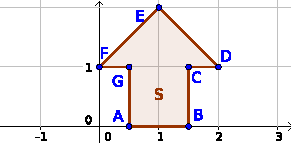
\includegraphics[width=7.0cm]{img/prova-3-pro-plano-1}
\hspace{1cm}
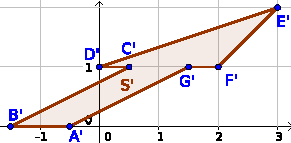
\includegraphics[width=7.0cm]{img/prova-3-pro-plano-2}
\end{center}
\Answer \fixme

\Exercise[title={2,5}] Seja $T: P_2 \to \R$ uma transformação linear.
\begin{enumerate}
\item É possível saber se $T$ é bijetora sem conhecer a sua regra/fórmula? Por que?
\item Supondo que $T( q(x) ) = q^{\prime}(0)$, para todo $q \in P_2$, qual é o núcleo de $T$? E a imagem de $T$?
\end{enumerate}
\Answer \fixme

\Exercise[title={2,5}] Seja $T_1: \R^2 \to \R^2$ a transformação linear que rotaciona os vetores de $\R^2$ em torno da origem segundo um ângulo de $\pi/2$ no sentido anti-horário. Considere também a transformação linear $T_2: \R^3 \to \R^2$, definida por $T_2(x,y,z)=(x+y+z, -x-y-z)$
\begin{enumerate}
\item Obtenha a fórmula/regra para a composta $T_1 \circ T_2$, isto é, $T_1 (T_2(x,y))$.
\item É correto afirmar que $T_1 \circ T_2$ é injetora? E que ela é sobrejetora? Justifique suas respostas.
\end{enumerate}
\Answer \fixme

\Exercise[title={2,5}] Seja $L: M_{2 \times 2} \to M_{2 \times 2}$ dada por $L(X) = X^T$. Obtenha as matrizes $[L]^\alpha_\alpha$ e $[L^{-1}]^\alpha_\alpha$, considerando a base $\alpha = \left\{ 
\begin{bmatrix}
3 & 0 \\ 0 & 0
\end{bmatrix},
\begin{bmatrix}
0 & 1 \\ 0 & 0
\end{bmatrix},
\begin{bmatrix}
0 & 0 \\ 4 & 0
\end{bmatrix},
\begin{bmatrix}
0 & 0 \\ 0 & 1
\end{bmatrix}
\right\}$ e calcule $[L(X)]_\alpha$, se $X = \begin{bmatrix}
2 & 7 \\ 1 & 8
\end{bmatrix}$.
\Answer \fixme
\end{ExerciseList}

\begin{center}
BOA PROVA!
\end{center}

%\newpage
%\restoregeometry
%\section*{Respostas}
%\shipoutAnswer
\end{document}
